\documentclass[a4paper,twoside,10pt]{report}
\usepackage[english]{babel}
\usepackage[utf8]{inputenc}
\usepackage{graphicx}
\usepackage{url}
\usepackage[export]{adjustbox}
\usepackage{indentfirst}
% pdflatex

% redefinição das margens das páginas
\setlength{\textheight}{24.00cm}
\setlength{\textwidth}{15.50cm}
\setlength{\topmargin}{0.35cm}
\setlength{\headheight}{0cm}
\setlength{\headsep}{0cm}
\setlength{\oddsidemargin}{0.25cm}
\setlength{\evensidemargin}{0.25cm}

\begin{document}

\begin{figure}[t]
\resizebox{60mm}{!}{
\includegraphics[left]{logoISEL.png}}
\end{figure}

\title{\huge\textbf{Lean Dashboard}}

\author{
\begin{tabular}{c}
José Pedro Jesus, n.º 44805\\
Hugo Manuel Jacinto Pinheiro, n.º 44886\\
Tomás Simão Mendes dos Santos, n.º 45363\\
\end{tabular}
}

\date{
\begin{tabular}{ll}
  {\textbf{Orientadores:}} & João Pereira, e-mail: joao.pereira@inetum.world, Inetum \\
                 & Filipe Freitas, e-mail: ffreitas@cc.isel.ipl.pt\\
\end{tabular}\\
\vspace{5mm}
\textbf{June 6th 2021 - V1 }}


\maketitle

\pagebreak
\tableofcontents{}
\newpage


\chapter{Introduction}

\section{Background}
Nowadays, within a company, it is even more important to have an organized and cooperative team with knowledge of all the steps and goals that need to be worked on for the various projects they are currently participating in.
Each member of the team must keep track of high amounts of information and since it is not uncommon that when working on a project a couple of platforms are used to keep track and share work done by the various members, useful information can be scattered on a vast amount of platforms, and sometimes even inside a single platform.
The information relative to a project can be obtained from different sources and it is all aggregated in one place, readily available to be displayed to a work team to better guide a certain project's development.

\section{Relevancy}
The Lean Dashboard Project will be developed to help the company's workers keeping track of all the possible tasks for their projects, gathering all the information needed for the various activities from the many sources that are necessary, presenting it on an easy to read and reactive web application.
The project at hands will be developed in partnership with Inetum\cite{INETUM} and will centre around the development of a responsive web application capable of running on a multitude of devices, ranging from smartphones to desktop computers to large screens such as TV’s. This web application will display to a work team of a company all the information regarding various projects being worked on. 
The information being displayed will show the team what needs to be addressed in the project at hands, such as milestones, bugs, and current errors in the project.

\section{Report Organization}
In this report, we will explain the early drafts of the implemented solution to the problem at hands, as well as provide a more in-depth analysis of the architecture and technology choices.

\chapter{Solution}

\section{Functionalities}
The solution will be a responsive mobile-first web application that will allow to consult and aggregate the information of various platforms. Inside a project, a manager will be able to add various dashboards that will then have the desired widgets. The widgets are the structures that hold and show the desired information regarding issues, tests, and sprints from platforms such as Jira, Squash and Azure. A manager will then be able to add various users to its project so that those users can consult all the dashboards with the relevant information in each widget.
\subsection{Implemented functionalities}
\begin{itemize}
    \item Retrieving the data from the multiple APIs
    \item Transforming the retrieved data in a widget format
    \item Creating a widget and adding it to an existing dashboard
    \item Updating widgets with the use of a scheduler
    \item Creating new projects
    \item Creating various Dashboards inside an existing project
    \item Partial authentication (creation of a local user, login, and logout)
    \item Lean Dashboard API partially implemented.
    \item RBAC roles and permission
    \item Setting the credentials for all the platforms
\end{itemize}

\newpage
\subsection{Research and planning}
\begin{itemize}
    \item Digital prototype of the front end
    \item Red routes diagram
    \item Information architecture (Website Map)
    \item Study of the React technology
\end{itemize}

\subsection{Functionalities to be added}
\begin{itemize}
    \item Finishing management of projects by the back-office manager
    \item Full authentication and authorization
    \item Revisiting the structure of widgets
    \item Finishing the client application
\end{itemize}

\section{Architecture}
\subsection{Architecture Principles}
The software solution being developed in the Lean Dashboard is divided into three main components: the ETL\cite{ETLPROC}, the Lean Dashboard Server and the client application.
\\ \newline
The ETL component, which stands for Extract, Transform and Load,  is responsible for obtaining the information from the various APIs and then transforming it to the desired format, widgets, and then proceeding to store them in a database. Both the topics of widgets and the storage solution being used will be addressed in this report in the Data model.
\\ \newline
With the use of the ETL procedure in our application, we bring a couple of advantages to the way we interact with the data being displayed.
\\ \newline
Since having near-real-time information is enough, with the Extract component we can avoid making high amounts of requests to the various APIs and avoiding overload them.
\\ \newline
Additionally, by adapting the extracted information (the Transform component) we can have a format of data that closely resembles the type and aspect of details we are trying the show to the user in each widget (we will also showcase the aspect of a widget in our application).
\\ \newline
Finally, with the information transformed to the desired format, when can then use a No-SQL database to store it and later decide how we will display it to the users 
\\ \newline
The Lean Dashboard server ends up serving as a gatherer of information. Inside this server, we will have all of the various projects, created by users, and each one will have its dashboards. Dashboards will be used to group the various widgets, and the user is the one to choose which dashboards will contain which widgets (these being the same widgets that we're created by the Extract, Transform and Load procedure)
\\ \newline
Lastly, we have the client application. The client application will be responsible for showing the user all of its projects. Users (if they are given these permissions) will be able to consult but also edit projects and dashboards. The main goal will be checking on the widgets inside a certain dashboard since those are the objects that contain the information being retrieved and transformed by the ETL.

\newpage
\subsection{Software Architecture}

\begin{center}
    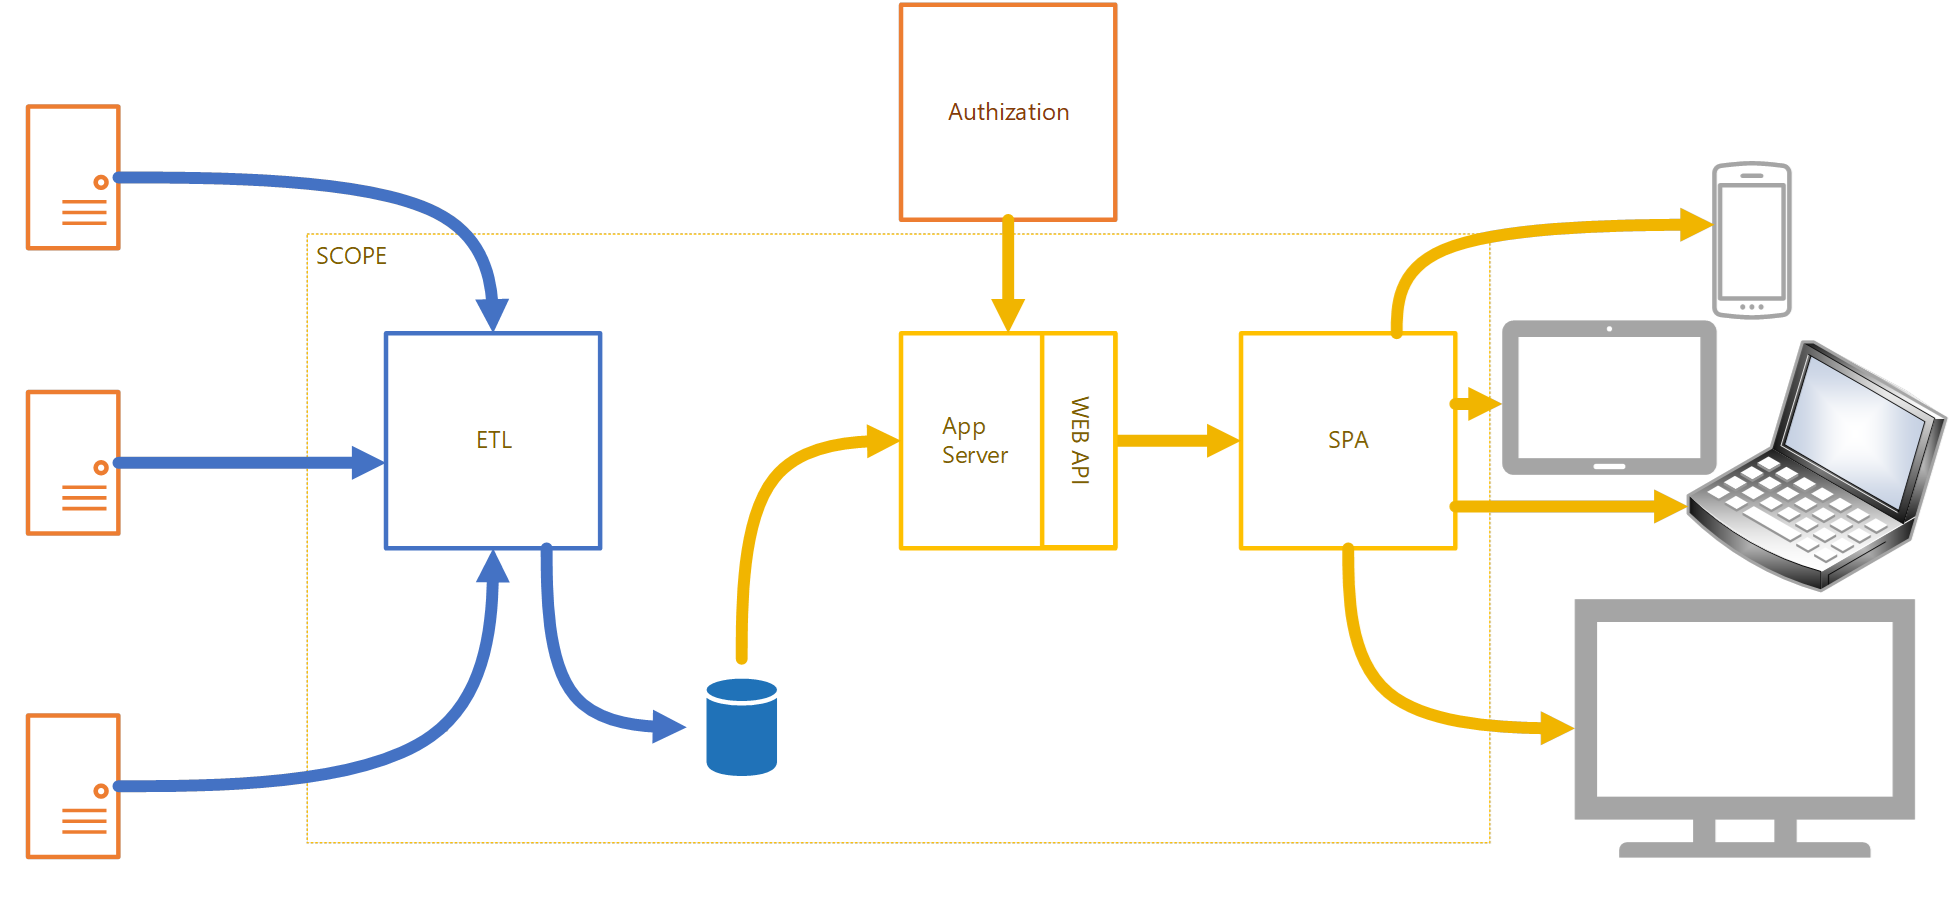
\includegraphics[width=\textwidth]{lean-dashboard-software-architecture.png}
\end{center}

*Explicação do esquema*

\subsection{Scheme of the back-end}
\begin{center}
    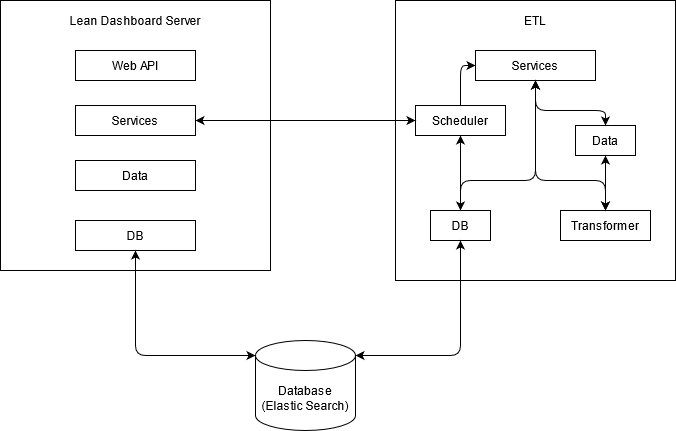
\includegraphics[width=\textwidth]{arquitetura_software.png}
\end{center}
*explicação dos módulos e da sua interação*

\newpage
\section{Data Model}
For the Data model and the storage of the information, we chose the No-SQL database Elastic Search.
\\ \newline
To better facilitate the getting and storage of information, we divided each object into they're own index, as displayed in the following scheme:
\begin{center}
    \resizebox{120mm}{!}{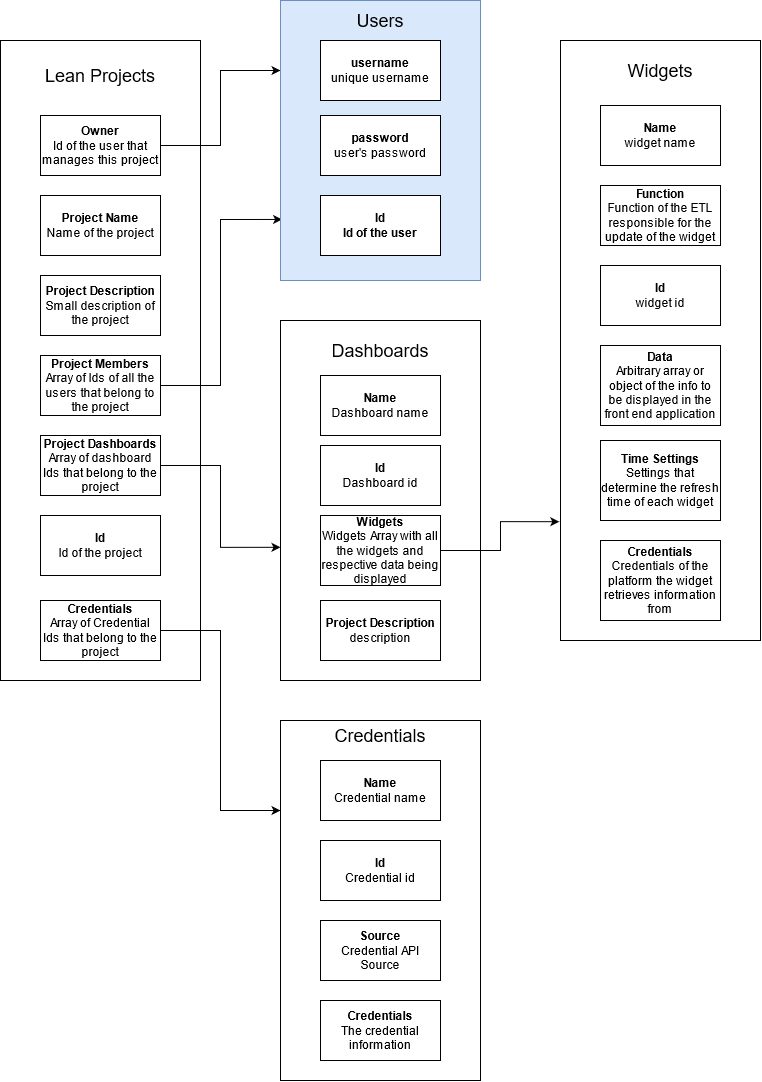
\includegraphics[width=\textwidth]{modelo de dados.png}}
\end{center}
*Texto a descrever os detalhes dos vários objetos*

\section{Authization module, Backoffice and Access control}
*Nesta secção iríamos explicar a utilização do módulo Authization, bem como as capacidades de gestão de backoffice a ser utilizadas e o controlo de acessos*

\chapter{User Experience Research}

\section{Red routes diagram}
Red Routes are a technique of User experience research that consists of a matrix that helps to prioritise our content and functionality based on usefulness to most users. With that, we can establish with functionalities need to be addressed first and be given more attention, regarding the number of users and the number of times a certain functionality is used.
\\ \newline
\begin{center}
    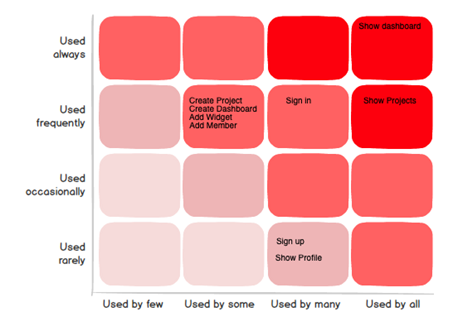
\includegraphics[width=\textwidth]{red-routes-diagram.png}
\end{center}
\newpage

\section{Information Architecture}
To better organize and structure the flow and various paths of our web application, we made our Information Architecture schema using the platform Miro:
\\ \newline
\begin{center}
    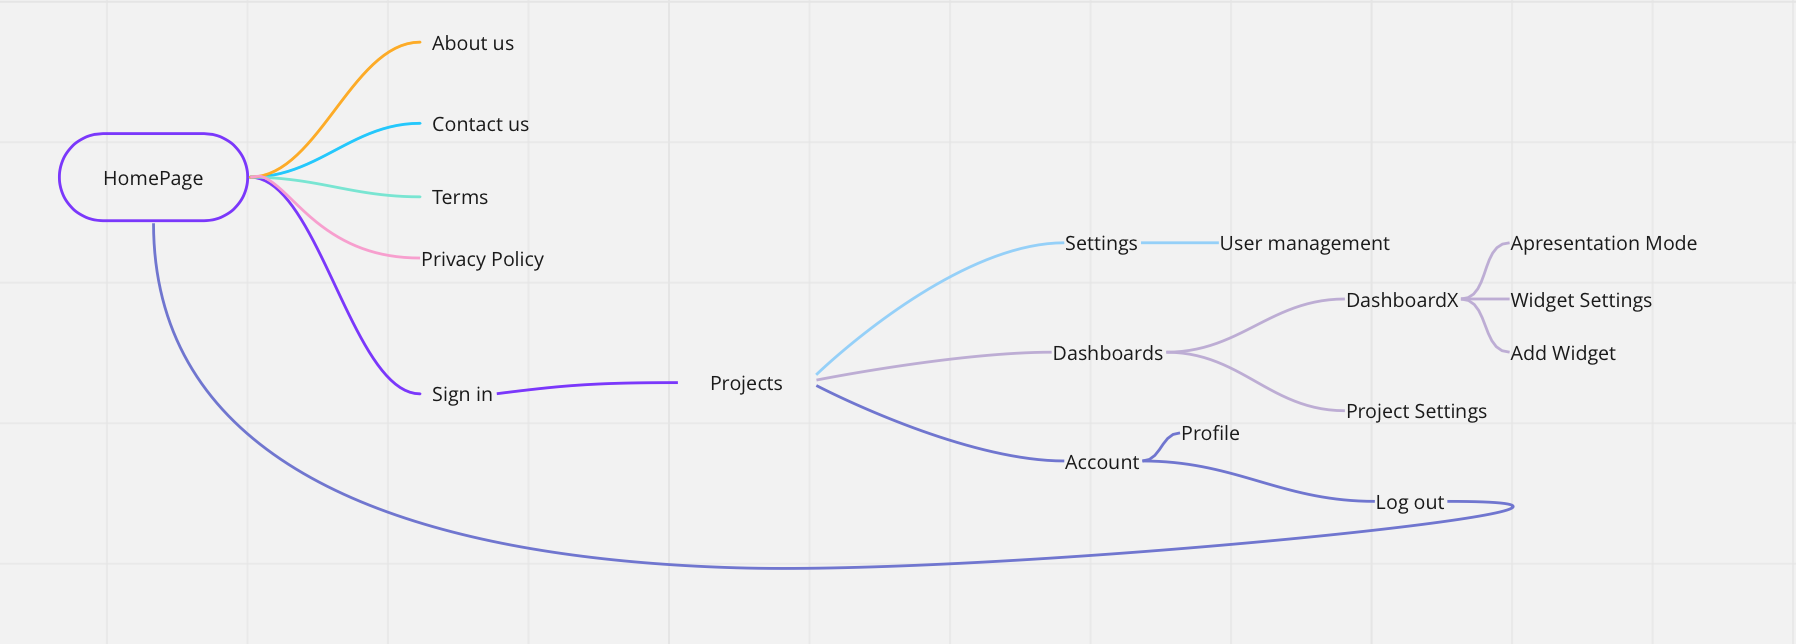
\includegraphics[width=\textwidth]{information-architecture.png}
\end{center}

With this diagram, we can better plan the making to the various resources by achieving a flowchart that dictates if the various flowchart accesses make sense (and easily correct them if they don't)

\section{Digital Prototype}
A Digital Prototype is a tool used in UI research to develop a mock user interface that can be utilized in use-case tests. These tests gather a small group of people and establish a task that all users need to complete. 
With the obtained results, we can then determine what aspects need to be addressed in the Digital Prototype by us developed.
This research and planning done beforehand (before the full implementation of the client application) can greatly decrease implementation costs since it is much easier to make modifications to this mocked user interface than it is to make some of the same changes on the client application code.
We utilized the platform Figma\cite{FIGMA} to develop our Digital Prototype, this being the prototype obtained:
\\ \newline
\begin{center}
    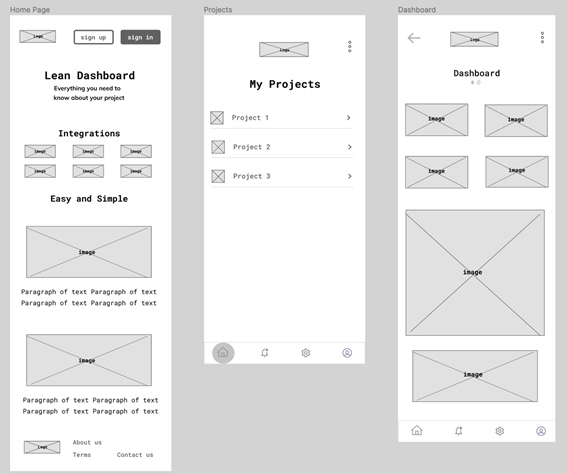
\includegraphics[width=\textwidth]{digital-prototype.png}
\end{center}

\chapter{Client Application}
*Nesta secção iríamos explicar alguns príncipios da aplicação cliente, bem como mostrar algumas das páginas por nós já feitas*

\begin{thebibliography} {websites}

\bibitem{INETUM} Inetum\\ https://gfi.world/pt-en/

\bibitem{ETLPROC} ETL - Understanding It and Effectively Using It.\\
https://medium.com/hashmapinc/etl-understanding-it-and-effectively-using-it-f827a5b3e54d\\
Consulted on April 1st 2021

\bibitem{MIRO} Miro - Platform used for the Information Architecture schema\\
https://miro.com/

\bibitem{REACT} React\\ https://reactjs.org/

\bibitem{FIGMA} Figma Prototype tool\\https://www.figma.com/prototyping/

\end{thebibliography} 

\end{document}